\documentclass[11pt]{article}

%%%%%%%%%%%%
% Packages %
%%%%%%%%%%%%

\hyphenpenalty=10000
\usepackage{tocloft}
\renewcommand\cftsecleader{\cftdotfill{\cftdotsep}}
\def\undertilde#1{\mathord{\vtop{\ialign{##\crcr
$\hfil\displaystyle{#1}\hfil$\crcr\noalign{\kern1.5pt\nointerlineskip}
$\hfil\tilde{}\hfil$\crcr\noalign{\kern1.5pt}}}}}
\usepackage{cleveref}
\usepackage{xcolor}
\usepackage[colorlinks = true,
            linkcolor = blue,
            urlcolor  = blue,
            citecolor = blue,
            anchorcolor = blue]{hyperref}
\usepackage{epstopdf}
\usepackage{braket}
\usepackage{upgreek}
\usepackage{caption}
\usepackage{booktabs}
\usepackage{subcaption}
\usepackage{amssymb,latexsym,amsmath,gensymb}
\usepackage{latexsym}
\usepackage{graphicx}
\usepackage{float}
\usepackage{enumitem}
\usepackage{pdflscape}
\usepackage{url}
\usepackage{tikz, calc}
\usetikzlibrary{shapes.geometric, arrows, calc}
\tikzstyle{norm} = [rectangle, rounded corners, minimum width=2cm, minimum height=1cm,text centered, draw=black]
\tikzstyle{arrow} = [thick, ->, >=stealth]
\newcommand{\argmin}{\arg\!\min}
\providecommand{\e}[1]{\ensuremath{\times 10^{#1}}} 
\providecommand{\mb}[1]{\mathbf{#1}}
\providecommand{\mh}[1]{\mathbf{\hat{#1}}}
\providecommand{\bs}[1]{\boldsymbol{#1}} 
\providecommand{\intinf}{\int_{-\infty}^{\infty}}
\providecommand{\fig}[4]{
  % filename, width, caption, label
\begin{figure}[h]
 \captionsetup{width=1.0\linewidth}
 \centering
 \includegraphics[width = #2\textwidth]{#1}
 \caption{#3}
 \label{fig:#4}
\end{figure}
}

\newcommand{\tensor}[1]{\overset{\text{\tiny$\leftrightarrow$}}{\mb{#1}}}
\newcommand{\tunderbrace}[2]{\underbrace{#1}_{\textstyle#2}}
\providecommand{\figs}[7]{
  % filename1, filename2, caption1, caption2, label1, label2, shift
\begin{figure}[H]
\centering
\begin{minipage}[b]{.45\textwidth}
  \centering
  \includegraphics[width=1.0\linewidth]{#1}
  \captionsetup{justification=justified, singlelinecheck=true}
  \caption{#3}
  \label{fig:#5}
\end{minipage}
\hspace{2em}
\begin{minipage}[b]{.45\textwidth}
  \centering
  \includegraphics[width=1.0\linewidth]{#2}
  \vspace{#7em}
  \captionsetup{justification=justified}
  \caption{#4}
  \label{fig:#6}
\end{minipage}
\end{figure}
}
\makeatletter

\providecommand{\code}[1]{
\begin{center}
\lstinputlisting{#1}
\end{center}
}

\newcommand{\crefrangeconjunction}{--}
%%%%%%%%%%%
% Spacing %
%%%%%%%%%%%
% Margins
\usepackage[
top    = 1.5cm,
bottom = 1.5cm,
left   = 1.5cm,
right  = 1.5cm]{geometry}

% Indents, paragraph space
%\usepackage{parskip}
\setlength{\parskip}{1.5ex}

% Section spacing
\usepackage{titlesec}
\titlespacing*{\title}
{0pt}{0ex}{0ex}
\titlespacing*{\section}
{0pt}{0ex}{0ex}
\titlespacing*{\subsection}
{0pt}{0ex}{0ex}
\titlespacing*{\subsubsection}
{0pt}{0ex}{0ex}

% Line spacing
\linespread{1.1}

%%%%%%%%%%%%
% Document %
%%%%%%%%%%%%
\begin{document}
\title{\vspace{-2.5em} Ad-Hoc Coordinate Change Algorithm For The Split-Aperture\\
  Polarization Microscope \vspace{-1em}} \author{Talon
  Chandler}% and Patrick La Rivi\`ere}
\date{\vspace{-1em}\today\vspace{-1em}}
\maketitle
\section{Introduction}
The split-aperture polarization microscope can measure the azimuth orientation
of a single dipole in two rotated views. These notes describe an algorithm for
converting noise-corrupted azimuth orientations in two rotated views into the
azimuth and inclination orientation. We define the coordinates, outline the
algorithm, then show the error in the estimate with noise-free and noise-corrupted
measurements.

\section{Coordinates}
\begin{figure*}[h]
 \captionsetup{width=1.0\linewidth}
 \centering
 \begin{subfigure}[t]{0.33\textwidth}
   \centering
   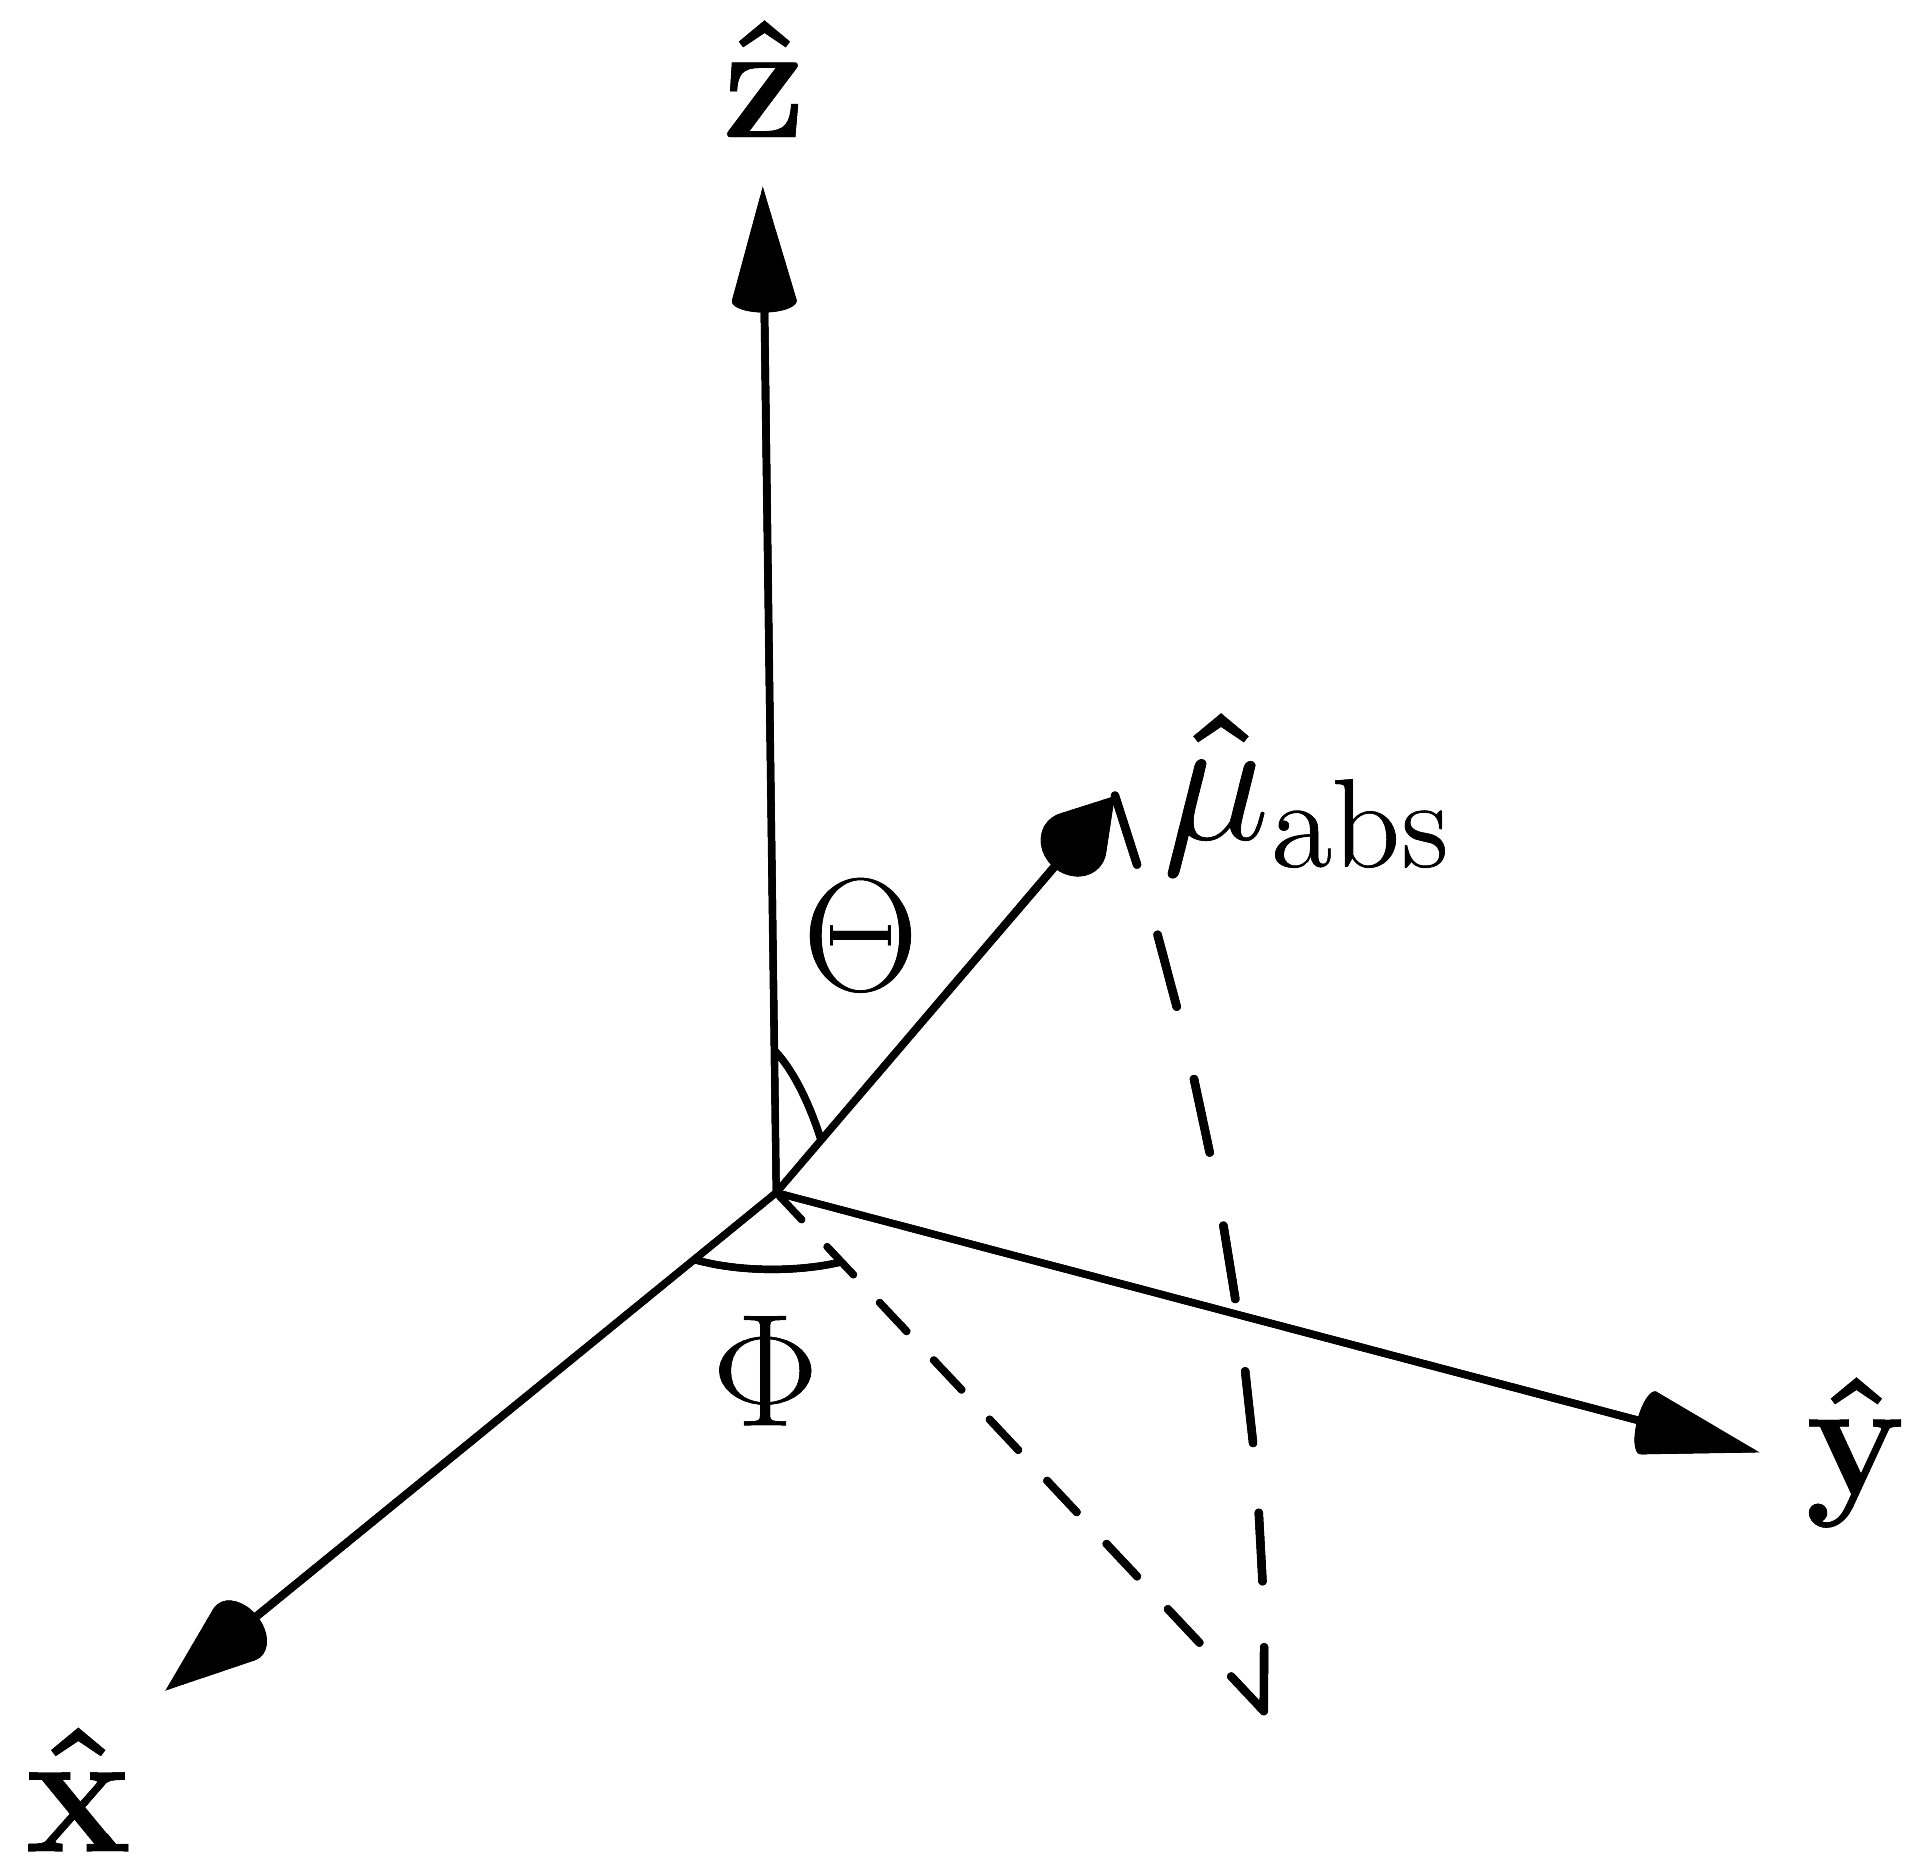
\includegraphics[width = 1.0\textwidth]{../figures/frame_a.pdf}
   \caption{$\theta$ and $\phi$ coordinate definitions.}
   \label{fig:frames_a}
 \end{subfigure}%
 ~
 \begin{subfigure}[t]{0.33\textwidth}
   \centering
   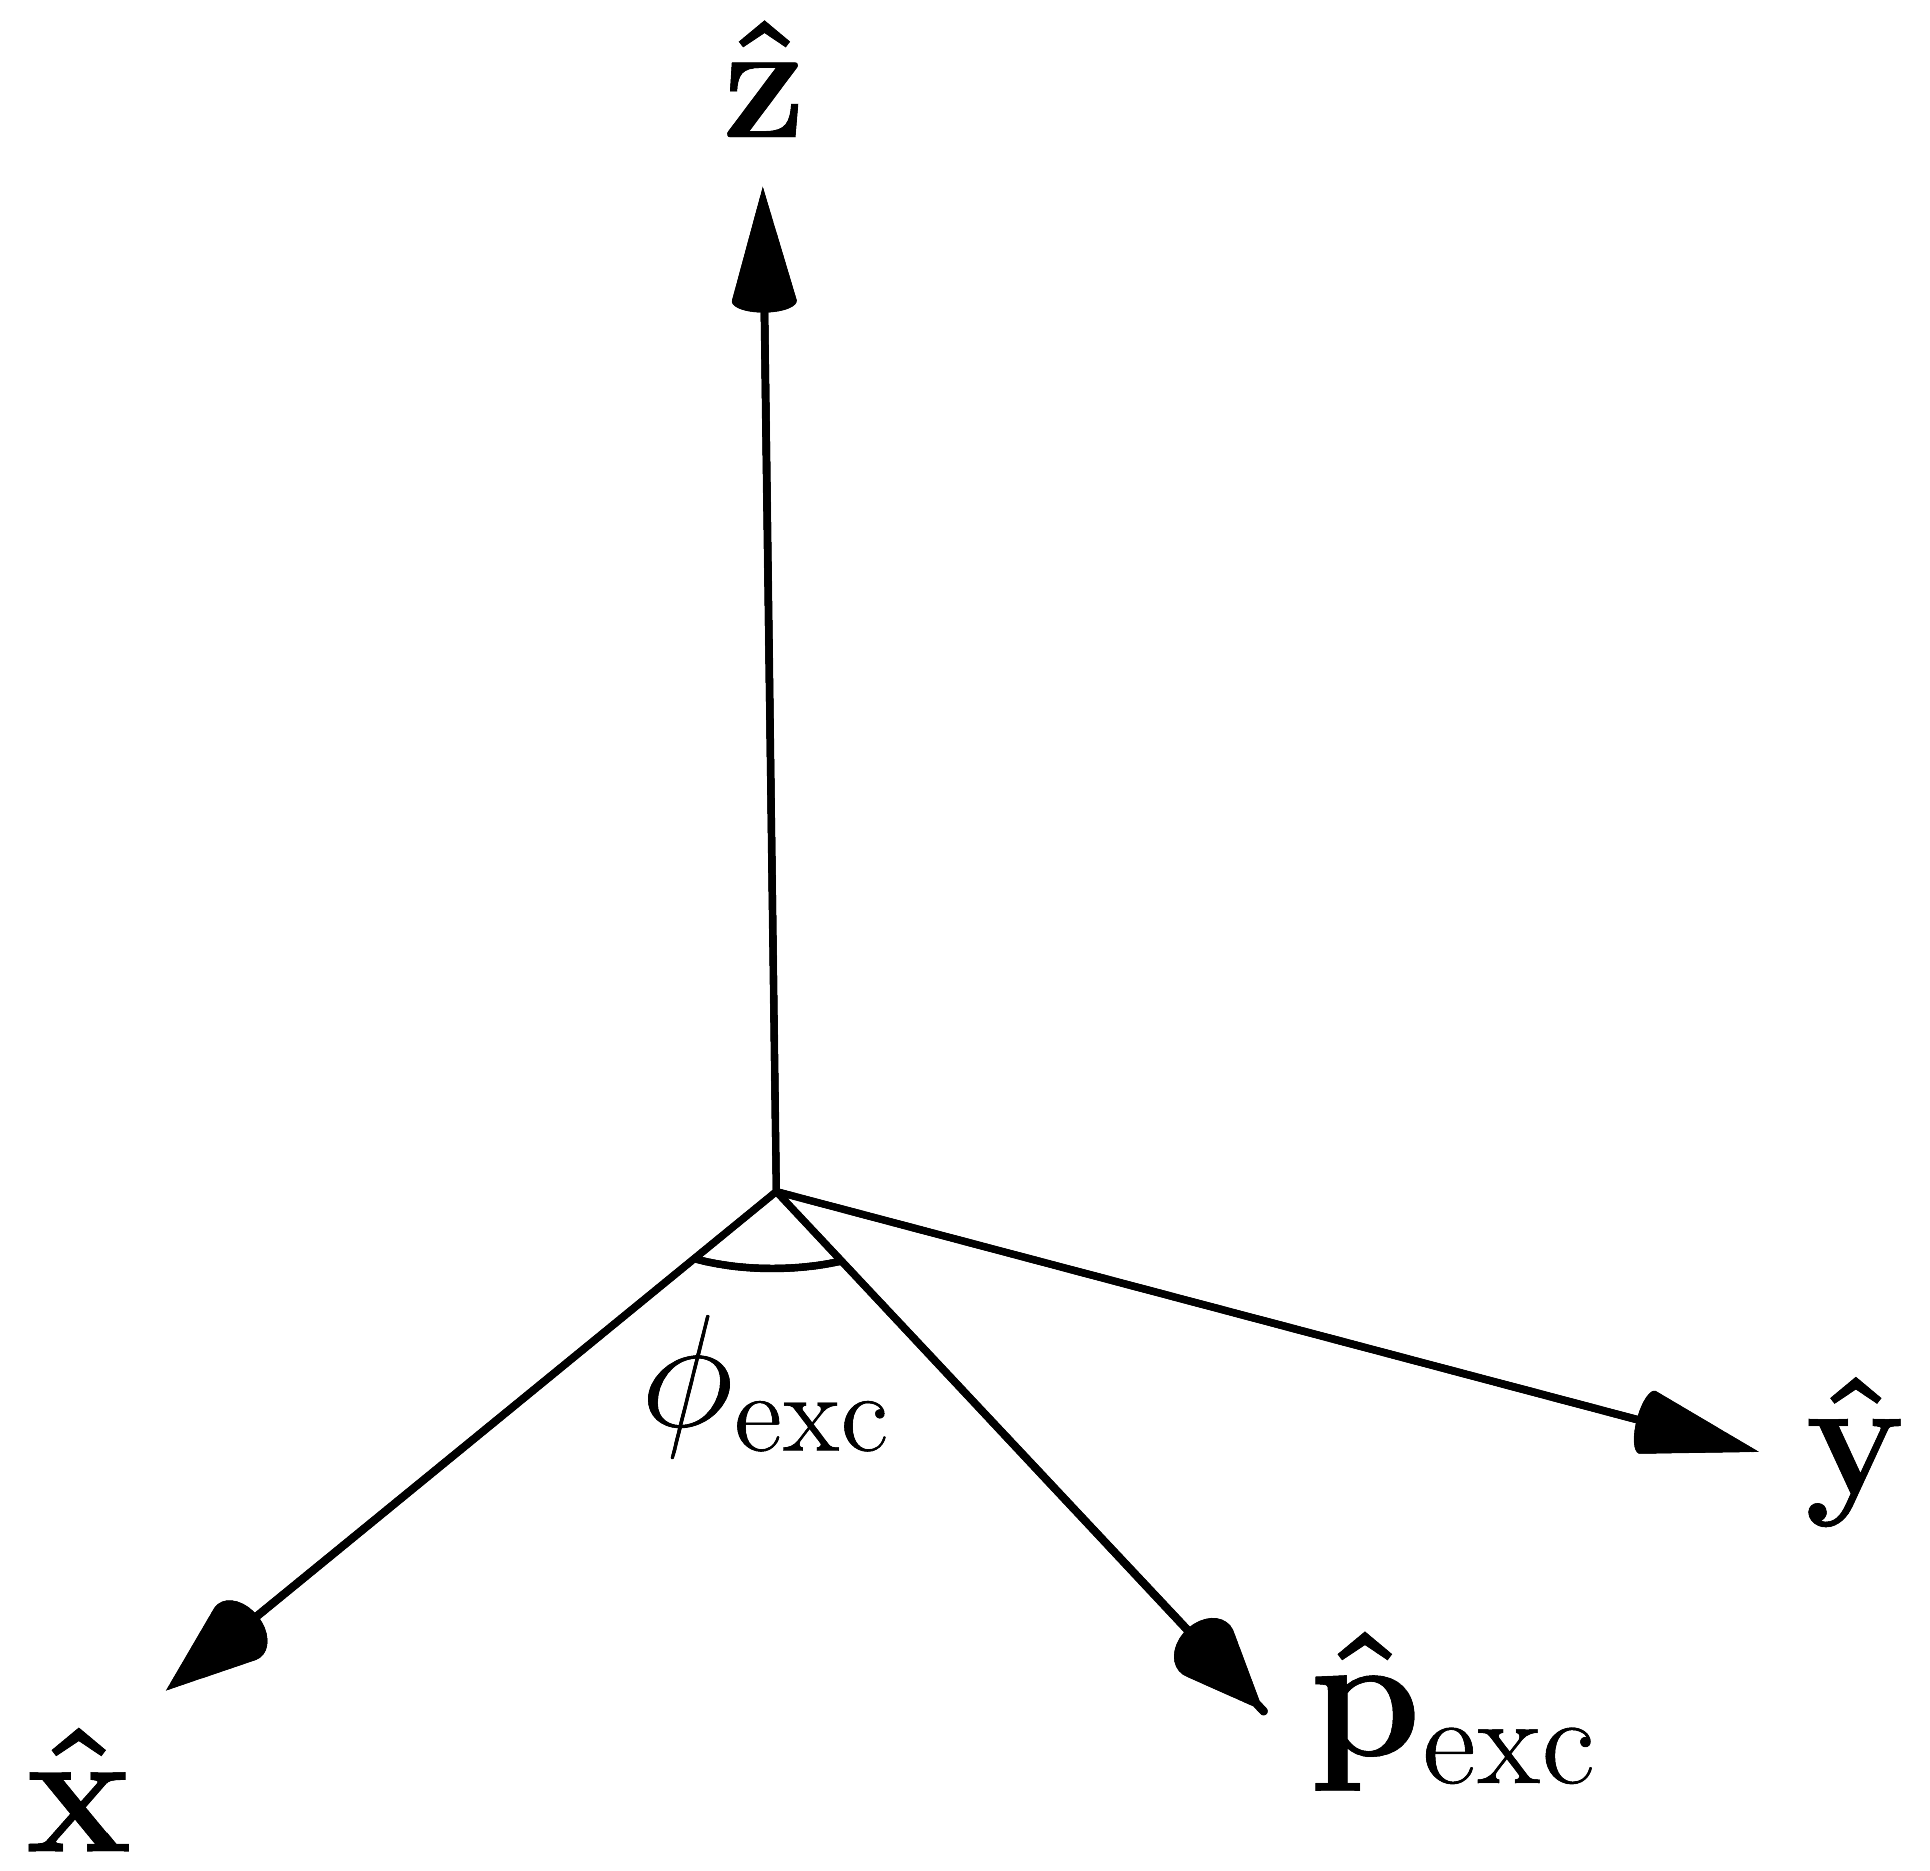
\includegraphics[width = 1.0\textwidth]{../figures/frame_b.pdf}
   \caption{$\phi'$ coordinate definition in the $+\alpha$ rotated frame.}
   \label{fig:frames_b}
 \end{subfigure}%
 ~
 \begin{subfigure}[t]{0.33\textwidth}
   \centering
   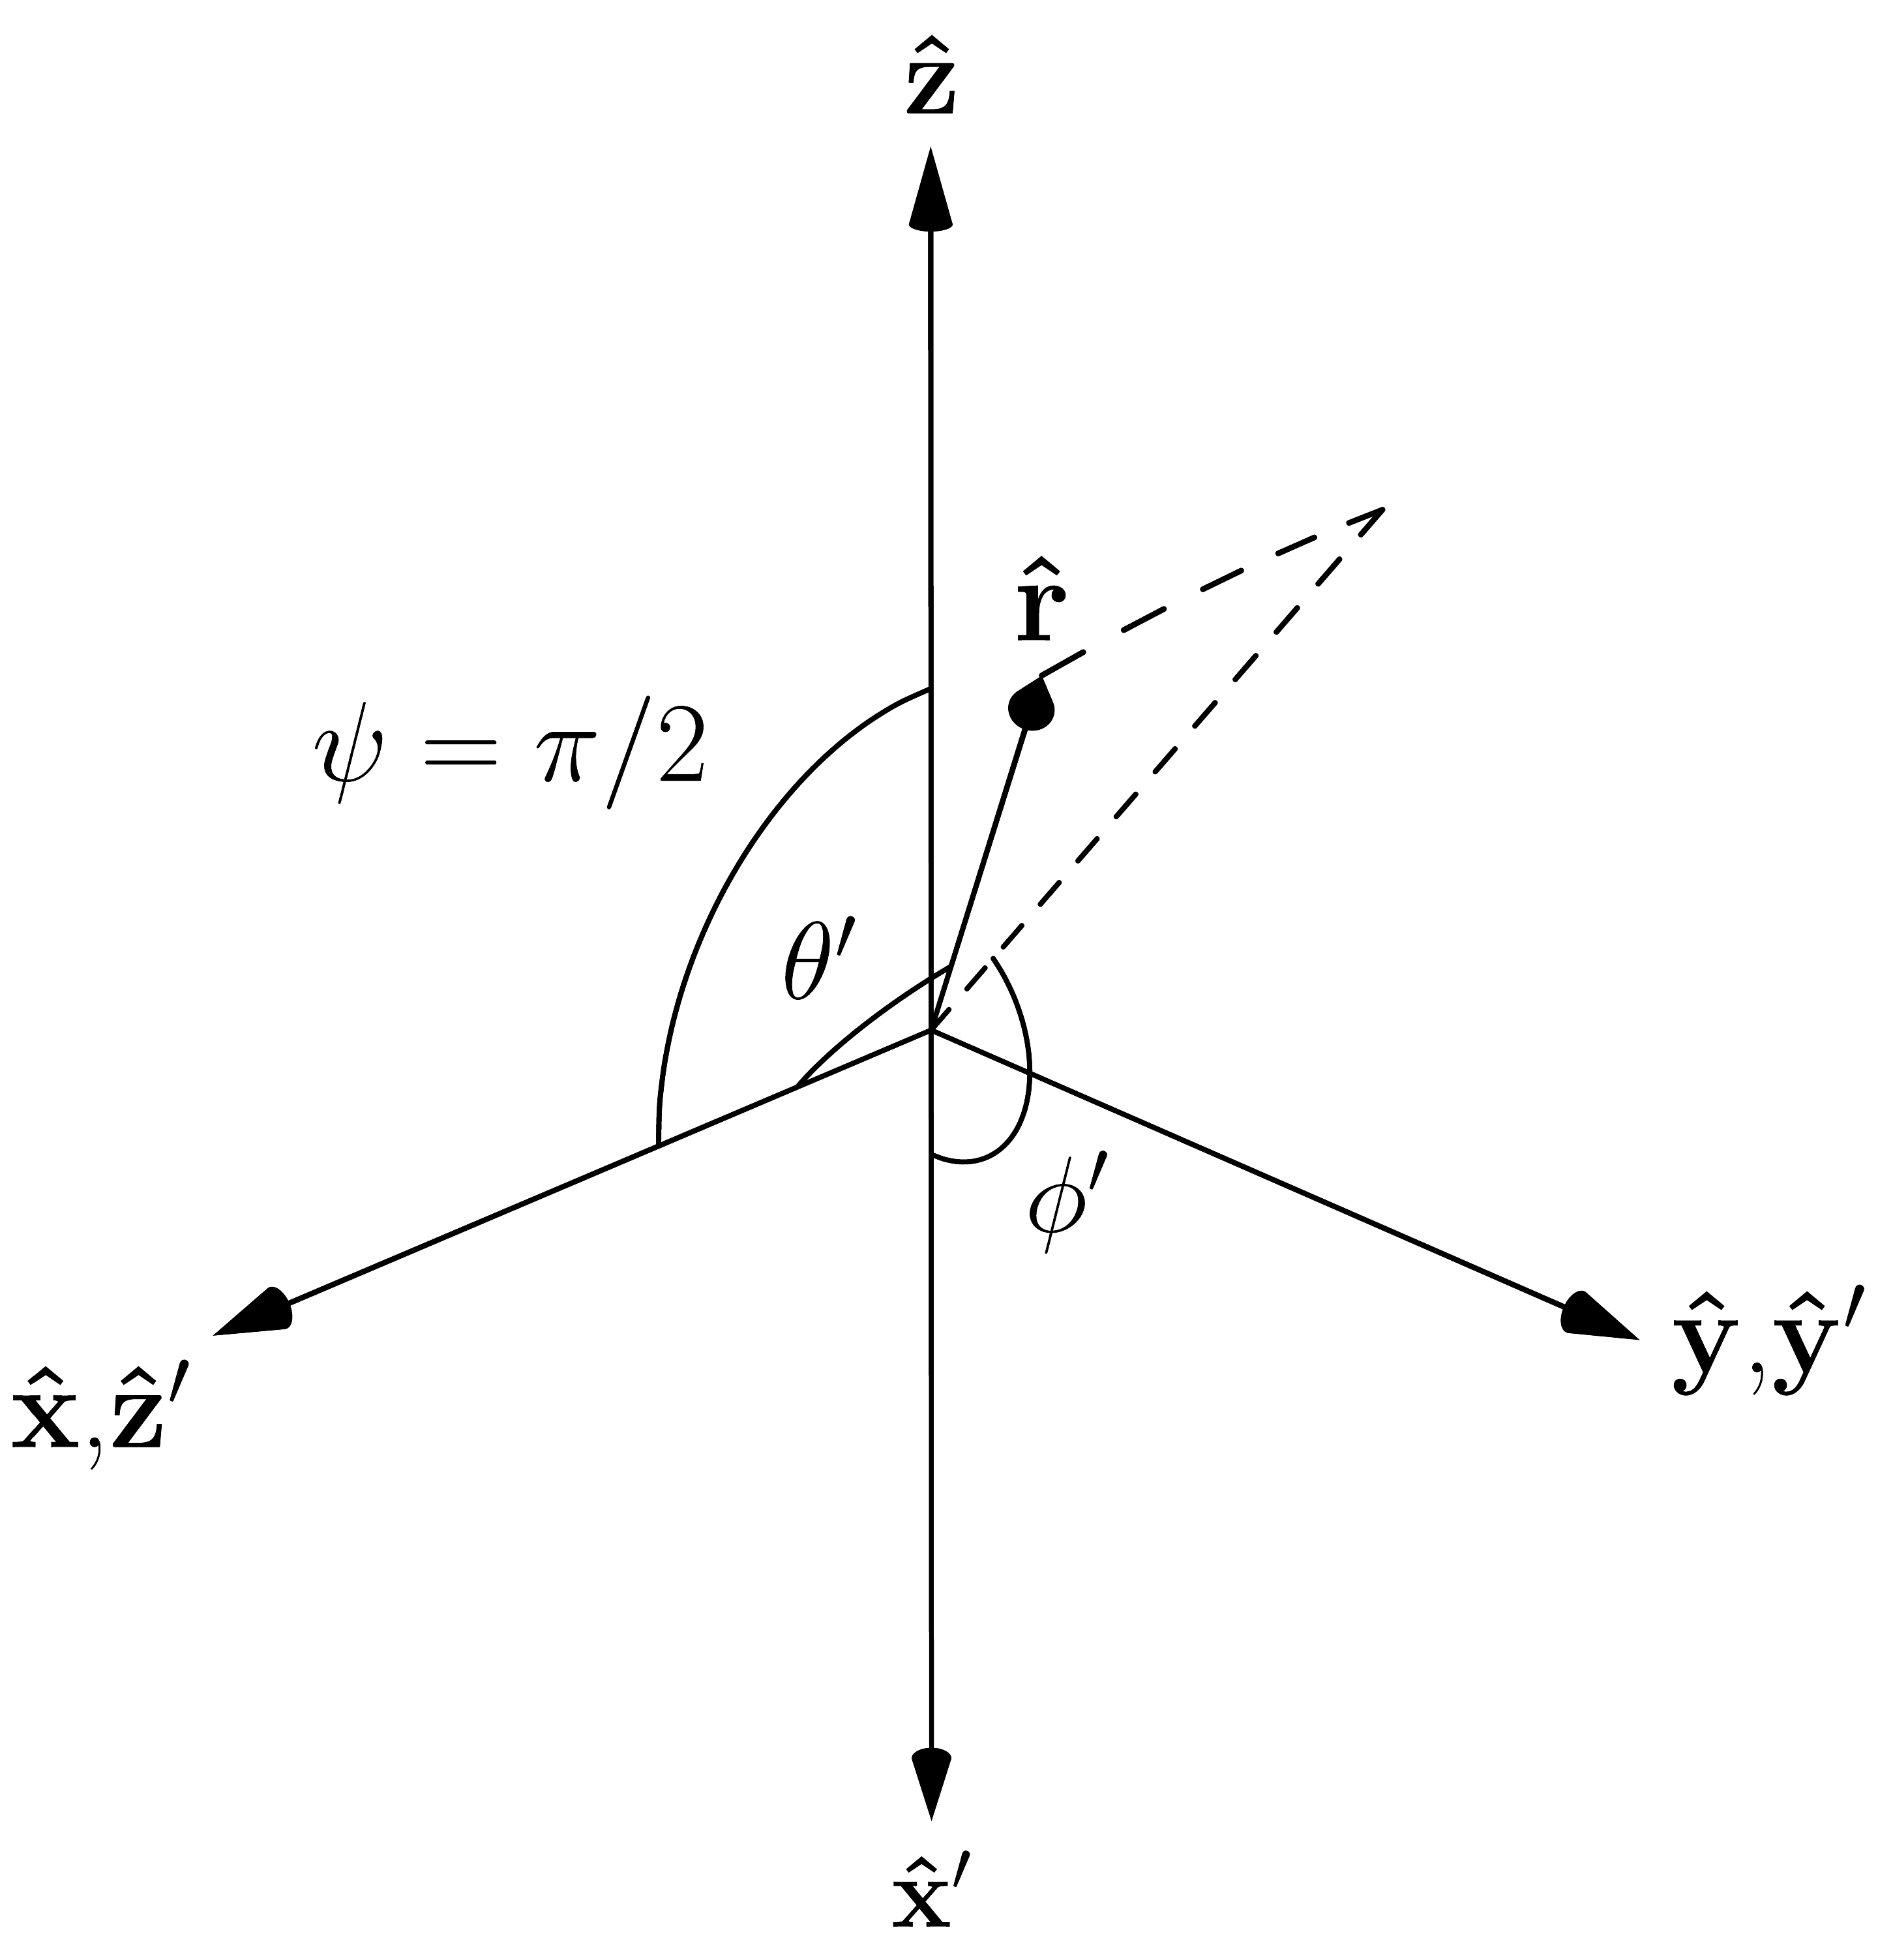
\includegraphics[width = 1.0\textwidth]{../figures/frame_c.pdf}
   \caption{$\phi''$ coordinate definition in the $-\alpha$ rotated frame.}
   \label{fig:frames_c}
 \end{subfigure}%
 \caption{Coordinate definitions.}
 \label{fig:frames}
\end{figure*}

Figure 1 shows one way of defining the inclination and azimuth angle in the
laboratory frame ($\theta$, $\phi$) and the azimuth angles in the rotated views
($\phi'$, $\phi''$). The two rotated frames are given by right-handed rotations
about the $+\mh{y}$ axis by an angle $\alpha$.

In
\href{https://github.com/talonchandler/dipsim/blob/master/notes/2017-06-09-rotated-frames/report/report.pdf}{previous
  notes} I have derived the relationships between the angles in Figure 1. We can
reuse those results and write:
\begin{align}
  \phi' &=
          \begin{cases}
            \arccos\left(\frac{\cos\alpha\cos\phi\sin\theta - \sin\alpha\cos\theta}{\sqrt{1 - (\sin\alpha\cos\phi\sin\theta + \cos\alpha\cos\theta)^2}}\right) \ \ \ &0 \leq \phi < \pi\\
            -\arccos\left(\frac{\cos\alpha\cos\phi\sin\theta - \sin\alpha\cos\theta}{\sqrt{1 - (\sin\alpha\cos\phi\sin\theta + \cos\alpha\cos\theta)^2}}\right) \ \ \ &-\pi \leq \phi < 0\\
            \end{cases}\\
  \phi'' &=
          \begin{cases}
            \arccos\left(\frac{\cos\alpha\cos\phi\sin\theta + \sin\alpha\cos\theta}{\sqrt{1 - (-\sin\alpha\cos\phi\sin\theta + \cos\alpha\cos\theta)^2}}\right) \ \ \ &0 \leq \phi < \pi\\
            -\arccos\left(\frac{\cos\alpha\cos\phi\sin\theta + \sin\alpha\cos\theta}{\sqrt{1 - (-\sin\alpha\cos\phi\sin\theta + \cos\alpha\cos\theta)^2}}\right) \ \ \ &-\pi \leq \phi < 0\\            
          \end{cases}.
\end{align}

\section{Procedure}
Equations 1 and 2 take $\theta$ and $\phi$ as input and give $\phi'$ and
$\phi''$ as output. We can rewrite equations 1 and 2 in operator form as
\begin{align}
  \mb{g} = \mathcal{H}\mb{f}
\end{align}
where $\mb{g} = [\phi', \phi'']$, $\mb{f} = [\theta, \phi]$, and $\mathcal{H}$
denotes the operation in equations 1 and 2. If there is noise introduced in the
measurement process then the model becomes
\begin{align}
  \mb{g} = \mathcal{H}\mb{f} + \mb{n}
\end{align}
where $\mb{n}$ is a noise vector.

Our task is to estimate $\mb{f}$ from noise-corrupted measurements $\mb{g}$. To
do so, we solve the following problem
\begin{align}
  \tilde{\mb{f}} = \argmin_{\mb{f}} ||\mb{g} - \mathcal{H}\mb{f}||_2 \label{eq:problem}
\end{align}
where $||\cdot||_2$ denotes the 2-norm. The search space of $\mb{f}$ is small
enough that a brute-force search is appropriate. First, we evaluate
$\mathcal{H}\mb{f}$ on a predetermined set of points to construct a lookup
table. When we take a measurement $\mb{g}$, we compute
$||\mb{g} - \mathcal{H}\mb{f}||_2$ at every point in the lookup table. Finally,
we choose the $\mb{f}$ that minimizes $||\mb{g} - \mathcal{H}\mb{f}||_2$ and
call that our estimate $\tilde{\mb{f}}$.

The samples used to construct the lookup table should be equally spaced if we
expect the lookup table procedure to introduce an equal amount of error into our
estimates. Note that $\mb{f}$ is a unit direction ($\mb{f}\in \mathbb{S}^2$) so
if we equally space the components of $\mb{f}$ ($\theta$ and $\phi$) most of the
sample points will be concentrated near the $\mb{z}$ axis. Instead of
constructing a lookup table with equally spaced $\theta$ and $\phi$ points, I
used approximately equally spaced points found using the
\href{http://stackoverflow.com/a/26127012/5854689}{Fibonnaci sphere algorithm}.

\section{Results}
I used $\alpha = 30^{\circ}$ for all tests.

To test the algorithm I chose 2000 equally spaced values of $\mb{f}$, calculated
$\mb{g} = \mathcal{H}\mb{f}$, then used the algorithm with a 500,000 point
lookup table to find $\tilde{\mb{f}}$. Finally, I found the error
$\mb{e} = |\tilde{\mb{f}} - \mb{f}|$ and plotted the individual components of
$\mb{e}$ in Figure 2.

The 2000 points I tested are not the same points as the lookup table points, so
the errors shown in Figure 2 are errors introduced by the lookup table
procedure. The error is different for different points because $\mathcal{H}$ is
nonlinear and because the points are varying distances from the lookup table
points. Each point in Figure 2 took $\sim 2$ ms to compute. We can trade speed
for accuracy in this algorithm by changing the number of points in the lookup
table.

I also performed the same test with noise-corrupted data. I chose 2000 equally
spaced values of $\mb{f}$, calculated $\mb{g} = \mathcal{H}\mb{f} + \mb{n}$
where $\mb{n}$ is a vector of Gaussian noise with $\mu = 0$ and
$\sigma = 2^\circ$, then used the algorithm with a 500,000 point lookup table to
find $\tilde{\mb{f}}$. Again, I found the error
$\mb{e} = |\tilde{\mb{f}} - \mb{f}|$ and plotted the individual components of
$\mb{e}$ in Figure 3.


\section{Limitations}
Using a precomputed lookup table will always introduce a varying amount of error
for different dipole orientations. If we want to have a constant error for all
dipole orientations, we could investigate iterative solutions that will stop
after a convergence criteria is reached.
\pagebreak

This model assumes that
\begin{itemize}[nosep]
\item both views use a narrow detection NA (no D-shaped aperture effects)
\item the azimuth angles measured from both views are equally weighted
\item the noise on the azimuth angles is normally distributed
\end{itemize}

\fig{../figures/recon-error.pdf}{.9}{Error introduced by the algorithm with
  noise-free data.}{results}

\fig{../figures/recon-error-gauss.pdf}{.9}{Error in the estimate with
  noise-corrupted data. I assumed that the two azimuth angle measurements had normally distributed noise with $\mu = 0$ and $\sigma = 2^{\circ}$.}{results}
\end{document}

